\Main
\hspace{0pt}
\vfill

\begin{center}
ОСНОВНАЯ ЧАСТЬ
\end{center}

\vfill
\hspace{0pt}
\pagebreak

\chapter{Теоретическая часть}
\label{cha:ch_1}

\section{Классическая квантизация}

Чтобы ответить на вопрос, что такое квантизация и что она дает, следует рассмотреть классический вариант, который наиболее прост и популярен на текущий момент, но имеет несколько существенных недостатков.

Квантизация — процесс перевода  вещественных параметров нейронной сети в целочисленный формат ограниченной длины бит. В классическом варианте, подробно описанном в \cite{quantization}, производится преобразование всех действительных параметров (весов и входных значений) нейронной сети в целочисленное представление с размером в $8$ бит ($1$ байт) на параметр. При такой схеме квантизации каждое целое число $q \in \{ 0, ..., 255 \}$ обозначает число $\overline{f}$ на вещественной оси, определяемое по (1.1).

\begin{equation}
\overline{f} = s(q - zp)
\end{equation}


А оптимальное целое число, к которому квантуется произвольное число $f \in R$ будет определяться по (1.2).

\begin{equation}
q = round \left( \frac{f}{s} \right) + zp
\end{equation}

Как можно заметить, в данных преобразованиях присутствуют константы $s$ и $zp$, которые являются параметрами квантизации и используются для преобразования из float-pointing представления мощности континуума, к которому принадлежит число $f$,  в ограниченное множество целых $8$-битных чисел (integer), представителем которого является число $q$. Схема такого преобразования проиллюстрирована на рис.1.1, где показано, как для вещественных чисел определяются соответствующие им целые числа, а для квантизованных значений действительные числа, которые они представляют.

\begin{figure}[H]
    \begin{center}
        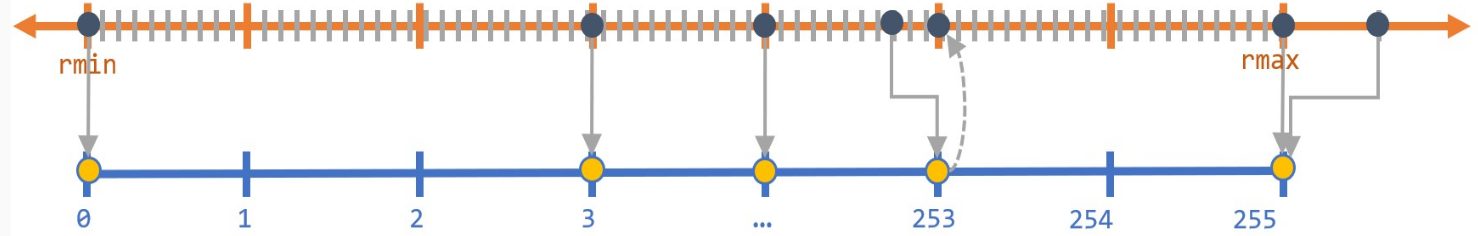
\includegraphics[scale=0.3]{inc/img/q8.jpg}
        \caption{Схема классической квантизации}
    \end{center}
\end{figure}

Будем называть уровнями квантизации вещественные значения, которые соответствуют всевозможным целочисленным квантизованным значениям $q$ параметра и определяются по формуле (1.1). Они обозначены оранжевыми штрихами на вещественной оси на рис.1.1.

Стоит обратить внимание на то, что в данной схеме $256$ уровней квантизации  распределены равномерно на отрезке минимального и максимального возможного значения параметра. Он определяется в процессе прогонки репрезентативной выборки реальных данных через исходную сеть. Процесс получения оптимальных  параметров квантизации для уже обученной модели при помощи прогонки через неё реальных данных, но без использования известных ответов, под которые обучалась сеть, будет называться в этой работе post-training квантизацией.

Перспективы, которые даёт квантизованное представление параметров:
\begin{itemize}
    \item Снижается объем вычислений за счет того, что операции сложения и умножения, которые используются в сетях, работают быстрее за счёт целочисленных вычислений и меньшего количества бит на одно число.
    \item Снижается размер, занимаемый сетью при вычислениях в оперативной памяти.
    \item Снижается размер, занимаемый сетью при хранении на жестком диске ЭВМ.
    \item Появляется возможность исполнения моделей на тех устройствах, в которых нет поддержки вещественной арифметики на уровне железа. Такими устройствами являются как микроконтроллеры компании ARM ниже версии Cortex Arm M4 в силу своей низкой стоимости и низкой производительности, так и высокоскоростные нейронные процессоры компаний Huawei и Qualcomm, которые берут на себя исполнение большинства нейронных сетей в современных телефонах и телевизорах. 
\end{itemize}

Однако очевидными являются и недостатки метода. Поскольку мощность поля вещественных чисел выше, чем ограниченного $2^K$ значениями множества целых чисел, где $K$ — количество бит для кодировки одного параметра,  легко догадаться, что данное преобразование будет вести к потерям точности работы обученной сети. Минимизация этой потери - основная задача инструмента, называемого квантизатором нейронных сетей, который выполняет это преобразование, подбирая наиболее оптимальные параметры квантизации $zp$ (zero point — точка, которой соответствует значение $0$ в вещественном поле) и $s$ (scale — коэффициент масштабирования). 

Равномерность распределения уровней квантизации является слабым местом классического алгоритма, поскольку распределение параметров в сети редко является равномерным, а имеет свою собственную природу, что будет показано далее. Этот факт является ограничителем для использования этого простого алгоритма для квантизации в представления с еще меньшим количеством бит, чем $8$, что демонстрируют результаты замеров, полученные в \cite{lq}, график которых показан на рис.1.2.

\begin{figure}[H]
    \begin{center}
        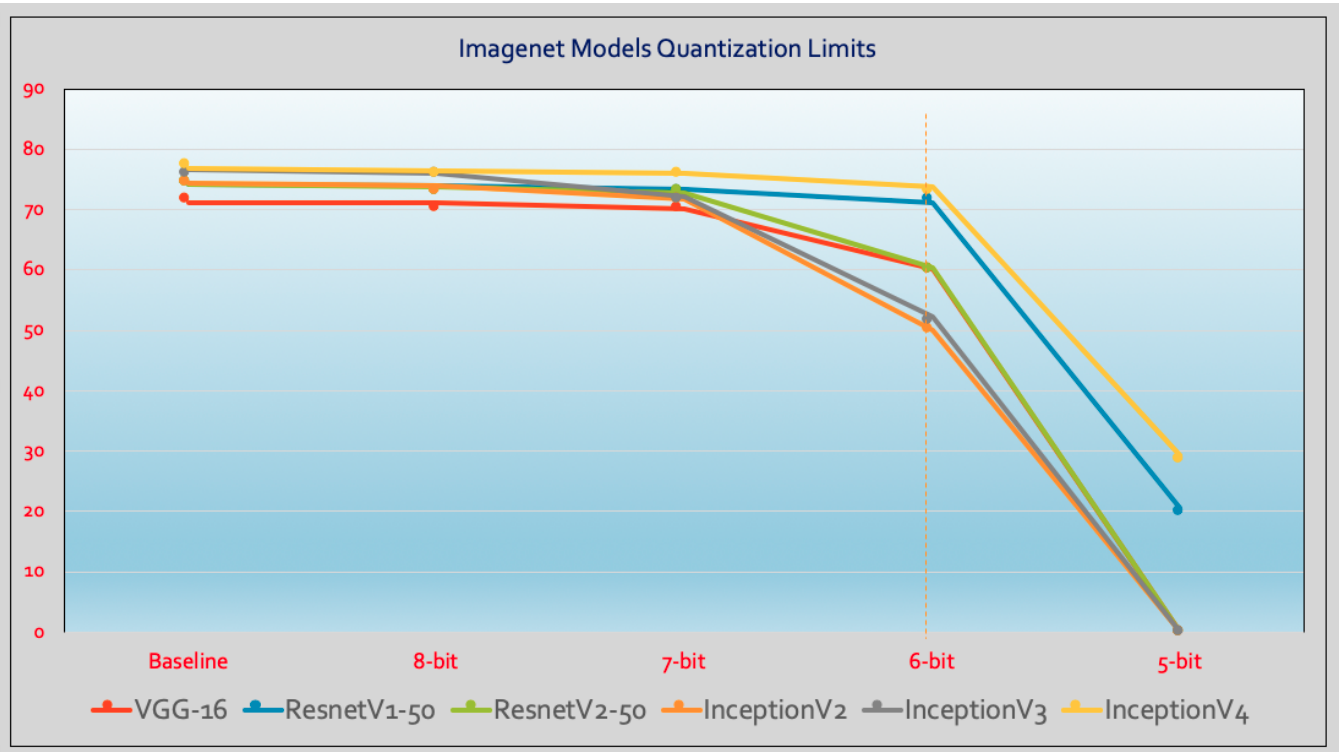
\includegraphics[scale=0.3]{tex/inc/img/q8stat.jpg}
        \caption{Точность моделей при уменьшении бит}
    \end{center}
\end{figure}

Этот же факт наталкивает на мысль о том, что для проведения более «экстремальной» квантизации с меньшим количеством бит на параметр, необходимо воспользоваться иными схемами интерпретации целого числа, которые будут лучше подстраивать уровни квантизации новой модели под распределение квантизуемых параметров. Именно о таком методе и будет идти речь в этой работе.

\section{Обучаемая квантизация}

Как уже было сказано выше, в данной работе вводится новый метод для квантизации сетей, который отличается от наиболее популярного и проверенного временем метода с равномерным распределением уровней квантизации. Перед предлагаемым алгоритмом квантизации, также как и перед любым другим, ставятся следующие задачи, которые он должен комплексно решать:

\begin{itemize}
    \item Определение оптимальных параметров квантизации как можно с меньшим количеством прогоняемых данных, затрачиваемых ресурсов и наибольшей сохраняемой  точностью модели.
    \item Возможность квантизации как можно в меньшие целочисленные размерности весов и активаций нейронной сети с целью уменьшения количества занимаемой памяти.
    \item Квантизация в такое представление, в котором эффективно производятся операции, тесно связанные с работой нейронных слоев, такие как перемножения матриц и свёртки.
\end{itemize}

По этой причине был выбран метод обучаемой низкобитовой post-training квантизации, который преобразует веса и активации глубокой модели в формат, позволяющий быстро и эффективно производить перемножения матриц при помощи побитовых операций. 

Суть этого метода заключается в том, что предлагается совершенно иной способ представления квантизованного числа в вещественом множестве. Обозначим кортеж $b = (b_0, b_1, ..., b_{K - 1}) \in \{ 0, 1 \}^K$ как бинарную запись квантизованного числа в Least Significant Bit first формате.  При классической квантизации одно $intK$ (где $K$ — количество бит для хранения одного значения) число $q$, вычисляемое по формуле (1.2), интерпретируется в действительном множестве как число $\overline{f}$ при помощи 2-ух параметров квантизации $s$ и $zp$ по формуле (1.1).

\begin{equation}
q = \sum \limits_{i = 0}^{K - 1} b_i 2^i
\end{equation}

В новом методе каждое квантизованное в $intK$ значение с бинарной записью $b$ интерпретируется согласно формуле (1.4), используя $a = (a_0, a_1, ..., a_{K-1})$ - вещественный базис-вектор коэффициентов для каждого из битов бинарного представления целого числа, имеющий длину $K$.

\begin{equation}
\overline{f} = \sum \limits_{i = 0}^{K - 1} b_i a_i,
\end{equation}

Иными словами, вещественное число, которое представлено квантизованным числом $q$ вычисляется как скалярное произведение базис-вектора из действительных чисел $a$ с бинарной записью этого квантизованного числа $b$. Базис-вектор $a$ будет являться настраиваемым параметром для отдельного слоя в процессе post-training квантизации. 

Следует оговориться, что из-за того,  что веса для каждого нейрона имеют разные распределения (что позволяет извлекать различные признаки из входных данных в рамках одного слоя), следует применять channel-wise квантизацию вместо layer-wise. Это означает наличие своего настраиваемого вещественного базис-вектора у каждого из нейронов слоя, вместо единого вектора для кодирования всех весов одного слоя.

С математической точки зрения это свойство не является обязательным, но в дальнейшем следует считать, что на значения базис-вектора $a$ накладывается строгое отношение частичного порядка: $a0 < a1 < ... < a_{K - 1}$. Это свойство дает возможность быстро определять отсортированные уровни квантизации <<на лету>>, что является важным свойством с при реализации.

Стоит отметить, что предлагаемый метод дает возможность интерпретировать биты числа не только в привычном множестве возможных значений $\{ 0, 1 \}$, но и в $\{ -1, 1 \}$, что позволяет уровням подстраиваться под отрицательные значения. Именно вариант $\{ -1, 1 \}$ будет использоваться в дальнейшем в данной работе. 

Описанная схема интерпретации числа $q$ на множестве действительных чисел имеет следующее преимущество: уровни квантизации накладываются не равномерно, а могут подстраиваться под конкретное распределение квантизуемого параметра. Например, если веса нейрона имеют стандартное распределение, то уровни квантизации должны иметь большую концентрацию  ближе к математическому ожиданию, что позволит точнее представлять величины, которые встречаются в сети наиболее часто. Пример вычисления и распределения уровней квантизации на числовой оси для $3$-х битной квантизации показан на рис.1.3.

\begin{figure}[H]
    \begin{center}
        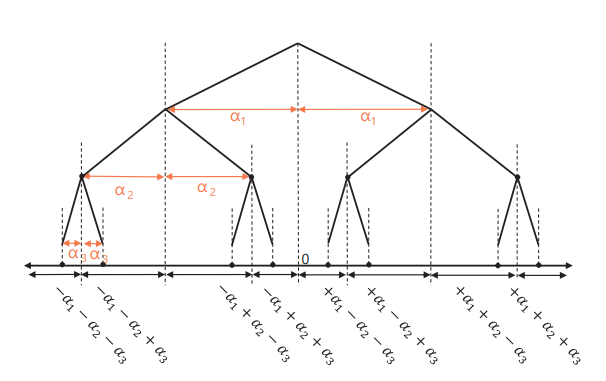
\includegraphics[scale=0.55]{tex/inc/img/lvls.jpg}
        \caption{Распределение уровней квантизации}
    \end{center}
\end{figure}

Если посмотреть на гистограмму весов в каналах слоёв нейронной сети для задач компьютерного зрения ResNet-20, полученное в работе \cite{lq}, становится понятно, что такой способ представления квантизованных значений точнее описывает генеральное распределение параметров.

\begin{figure}[H]
    \begin{center}
        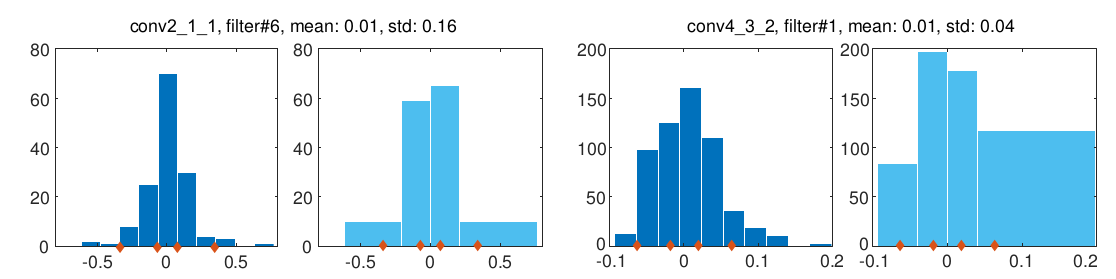
\includegraphics[scale=0.36]{tex/inc/img/distrib.jpg}
        \caption{Распределение весов в ResNet-20}
    \end{center}
\end{figure}


На рис. 1.4. точками оранжевого цвета показано, как можно оптимально разместить уровни при описанном способе кодировки вещественных величин для $2$-х битной квантизации весовых параметров. Следует обратить внимание на то, что веса в разных каналах слоя имеют разные распределения, что является обоснованием для выбора channel-wise преобразования вместо layer-wise, о чем было упомянуто выше.

Стоит не забыть упомянуть, что количество уровней квантизации для $intK$ равно $2^K$, а сами уровни получаются в результате применения формулы (1.4) ко всевозможным комбинациям бинарных записей из $K$ бит.

\begin{figure}[H]
    \begin{center}
        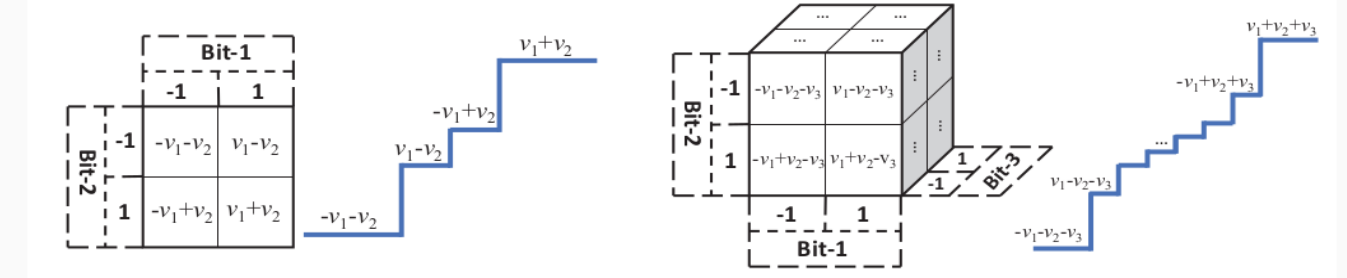
\includegraphics[scale=0.35]{tex/inc/img/lvls2.jpg}
        \caption{Уровни квантизации}
    \end{center}
\end{figure}

Возникает вопрос не только, как интерпретировать имеющееся квантизованное число в вещественном представлении, но и каким целочисленным значением оптимальнее всего представить число с действительной оси. Эта часть описываемого алгоритма идентична тому, как аналогичное преобразование производится для классической $8$-битной квантизации, однако стоит рассмотреть этот этап поподробнее. Сначала на основе базис-вектора $a$ определяются уровни квантизации $q_l = (a, e_l), \; \forall e_l \in \{ -1, 1 \}^K$, такие что $q_0 < q_1 < ... < q_{2^K}$, и на основе них рассчитываются пороги  $t_l = \displaystyle\frac{q_l + q_{l-1}}{2}$, с помощью которых определяется к какому уровню следует отнести конкретное число, как показано на рис.1.6. 

\begin{figure}[H]
    \begin{center}
        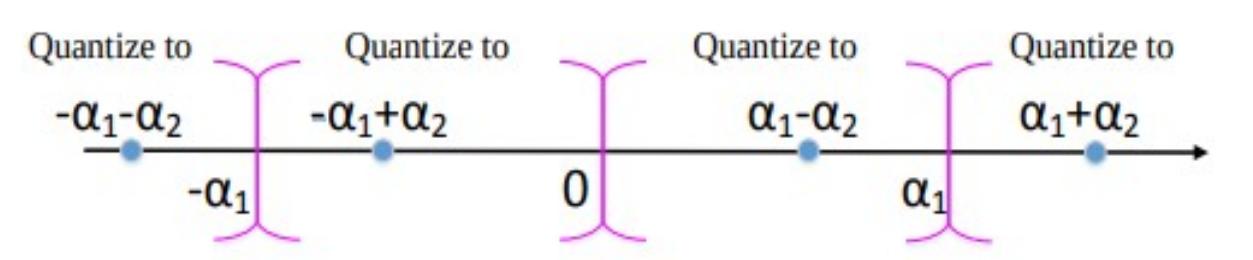
\includegraphics[scale=0.3]{tex/inc/img/define.jpg}
        \caption{Определение оптимальной кодировки}
    \end{center}
\end{figure}

После определения уровня квантизации  при помощи порогов, следует взять соответствующую бинарную кодировку, которая будет являться оптимальным квантизованным значением для исходного вещественного числа.

Для того, чтобы уровни могли распределяться не только вокруг $0$, но и любого другого числа (ведь распределение значений параметра может быть смёщенным), следует добавить свободный коэффициент смещения к обучаемому базис-вектору, что даст дополнительную степень свободы описываемому алгоритму. Однако исследование и решение этой проблемы не затрагивается в данной работе.

У метода есть явный недостаток — большое количество настраиваемых аргументов, равное сумме длин всех базис-векторов. Издержки на хранение таких векторов в памяти достаточно малы по сравнению с количеством весовых значений, поэтому их можно не брать в учет при анализе метода. Но обучение  при таком числе параметров квантизации становится трудной задачей, требующей применения различных эвристик, которые позволяют находить оптимумы в вещественных пространствах больших размерностей.

Как было заявлено и будет показано далее в описании работы нового слоя, такой вариант преобразования параметров даёт возможность быстрого матричного перемножения квантизованных весовых и входных значений. Среди огромного разнообразия существующих операций, встречающихся в глубоких моделях на текущий момент, наиболее ярко выделяются полносвязные слои, рекуррентные, свёрточные и субдискретизационные. Именно на работе этих операций построена любая современная нейронная сеть, поэтому на них следует делать упор при оптимизации работы моделей, в том числе и в квантизации. 

Упомянутые субдискретизационные слои являются довольно быстрой операцией, работающей за $O(n)$ от размера входных данных, и издержки на проведение квантизации с учётом потери точности слишком велики по сравнению с выгодой, которую может дать предлагаемое преобразование. Рекуррентные сети, такие как GRU, LSTM, RNN, описанные в \cite{gru}, \cite{lstm}, \cite{rnn} соответственно, содержат внутри своей реализации полносвязные нейронные слои. Что касается свёрточных слоев, про которые подробно рассказывается в \cite{conv}, то операция свёртки в них может быть сведена к перемножению двух матриц (GEMM) при помощи im2col преобразования. Эта техника, описанная в \cite{im2col}, зачастую применяется, поскольку позволяет добиться значительного увеличения скорости работы таких слоёв за счет того, что алгоритм перемножения матриц оптимальнее работает с кешом процессора, благодаря последовательному доступу к памяти.  Именно поэтому в данной работе было решено акцентировать внимание на проведение квантизации с классическим полносвязным слоем, поскольку все остальные существующие операции либо содержат такой слой внутри себя, либо могут быть приведены к такому формату, либо издержки и потери превалируют над возможным выигрышем от преобразования, поскольку не содержат в себе ресурсоёмких матричных произведений. Все слои сети, отличные от полносвязных, будут оставаться без изменений в данной работе.

Описанный в \cite{rnn} классический полносвязный нейронный слой — это набор из нейронов, реализующих в себе алгоритм линейной регрессии вместе с функцией активации, которая призвана добавить нелинейности к выходу нейрона и придать системе большую устойчивость за счет асимптотических ограничений, накладываемых на выход нейрона. Количество таких нейронов задается тем, кто обучает подобный слой. Как нетрудно догадаться, оно равно размерности выходного вектора (output), который выдает слой на основе входного вектора данных (input). Схематично нейрон сети может быть представлен схемой на рис. 1.7.

\begin{figure}[H]
    \begin{center}
        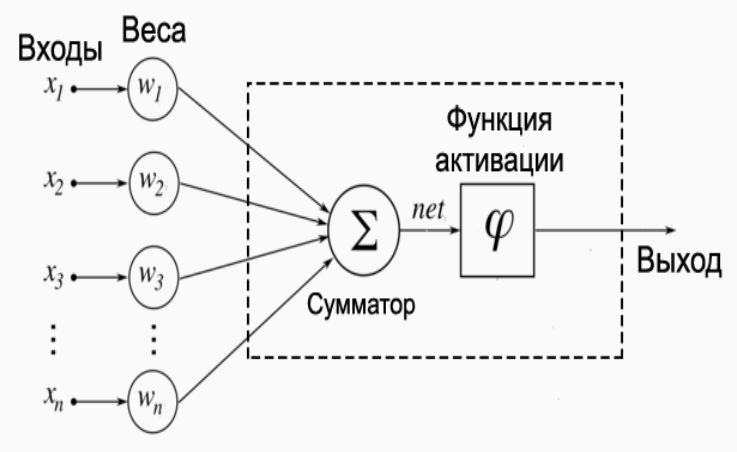
\includegraphics[scale=0.3]{tex/inc/img/neron.jpg}
        \caption{Нейрон}
    \end{center}
\end{figure}

В то же самое время показанная схема эквивалентна вычислению функции активации $\sigma$ от суммы между скалярным произведением входов слоя $x$ с вектором весов нейрона $w$ и смещением для $i$ - го нейрона по формуле (1.5).

\begin{equation}
y_i = \sigma((x_i, w_i) + b_i), \; \forall i: 0 < i < m
\end{equation}

Выход такого нейрона — скаляр $y_i$, называемый выходом нейрона.

Формулу (1.5) можно расширить в более общий случай, когда на вход поступает несколько входных векторов в виде матрицы $X$ и используется целый полносвязный нейронный слой из $m$ описанных выше нейронов, веса которых также могут быть объединены в единую матрицу $W$, столбцы в которой — весовые вектора для отдельного нейрона. Тогда выходную матрицу $y = (y_0, y_1, ..., y_{m - 1})$ можно рассчитать при помощи результата произведения матрицы весов на матрицу входов, к каждой строке которого добавляется вектор смещений $b = (b_0, b_1, ..., b_{m-1})$, состоящий из свободных коэффициентов каждого нейрона слоя, и поэлементно применяется функция активаций $\sigma$, что отображено в (1.6).

\begin{equation}
y = \sigma (XW + b)
\end{equation}

\begin{figure}[H]
    \begin{center}
        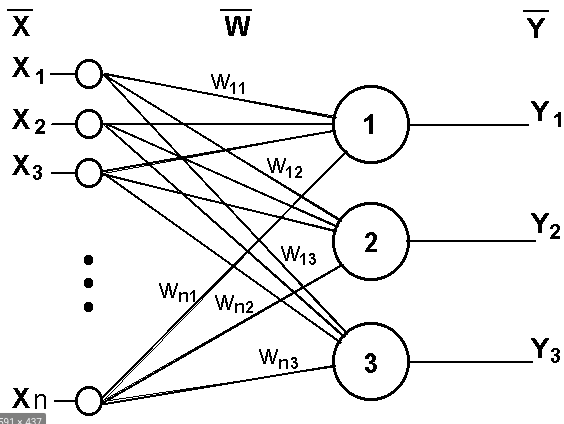
\includegraphics[scale=0.3]{tex/inc/img/layer.jpg}
        \caption{Полносвязный слой}
    \end{center}
\end{figure}

Основываясь на специфике работы слоя, проиллюстрированного рис. 1.8., можно выделить следующие параметры нейронного слоя, которые необходимо хранить и использовать при расчетах:

\begin{itemize}
    \item Веса модели в виде матрицы $W \in R^{n \times m}$, где $n$ - размер входных векторов, а $m$ - количество нейронов.
    \item Вектор из смещений всех нейронов $b \in R^{m}$.
    \item Тип функции активации $\sigma$, которая применяется к каждому значению выходного вектора.
\end{itemize}

Поскольку смещения занимают мало места в памяти и сложение происходит за $O(n)$, квантизовать их не имеет смысла. Зато весовые параметры составляют наибольшую часть занимаемого сетью объема, а время на перемножение весов на матрицу входов $X$ является самой ресурсоемкой операцией, оптимизировать которую можно в квантизованных вычислениях, используя побитовую арифметику. 

Как было показано выше, поскольку у каждого из нейронов свое распределение весов, то квантизовать следует каждый из его весовых векторов отдельно. При этом в данном методе затрачивается $K_w$ битов на квантизацию каждого веса нейрона. Тогда каждый весовой вектор нейрона может быть представлен бинарной матрицей $B^w \in \{ -1, 1\}^{K_w \times n}$, где каждому весу исходного вектора соответствует бинарный столбец, означающий его квантизованное значение.  Каждый входной вектор (строка матрицы $X$) также может быть представлен в бинарном виде $B^x \in \{ -1, 1 \}^{K_x \times n}$  при помощи отдельных параметров квантизации для входов слоя. Следует сразу отметить, что количество бит $K_w$ на кодирование весов может не совпадать с количеством $K_x$, используемым для кодирования входных значений.

В таком случае, результат скалярного произведения входного и весового вектора в квантизованных вычислениях будет расчитываться по формуле (1.7).

\begin{equation}
\sum\limits_{k = 1}^{n} x_k w_k \approx \sum\limits_{k = 1}^{n}\sum\limits_{i = 1}^{K^x} (b^x_{ik} a^x_i) \sum\limits_{j = 1}^{K^w} (b^w_{jk} a^w_j) = \sum\limits_{i = 1}^{K^x}\sum\limits_{j = 1}^{K^w} a^x_i a^w_j (\sum\limits_{k = 1}^{n} b^x_{ik} b^w_{jk}),
\end{equation}

где $b^x_{ik}$ и $b^w_{ik}$ - бит, находящийся на $i$-ой строке в $k$-ом столбце бинарной матрицы $B^x$ и $B^w$ соответственно. 

Обозначим $i$-ую строку бинарной матрицы $B^x$ и $B^w$ как $b^x_{i}$ и $b^w_{i}$ соответственно, а под оператором $\odot$ будем понимать скалярное произведение двух бинарных векторов. В таком случае формулу (1.7) можно переписать в виде (1.8).

\begin{equation}
\sum\limits_{k = 1}^{n} x_k w_k \approx \sum\limits_{i = 1}^{K^x}\sum\limits_{j = 1}^{K^w} a^x_i a^w_j (b^x_{i} \odot b^w_{j}),
\end{equation}

Для обоснования выигрыша в скорости, который дает предложенная формула для расчета, следует подробнее рассмотреть бинарное скалярное произведение.

 Скалярное произведение — сумма произведений соответствующих элементов двух векторов. В это же время бинарное множество $\{ -1, 1 \}$ замкнуто относительно операции умножения, поэтому произведение двух бинарных значений остается бинарным значением, а значит может быть представлено одним битом. Возможны следующие варианты произведения $2$-ух битов:

\begin{enumerate}[label=\arabic*.]
    \item $-1(0) \cdot -1(0) = 1(1)$
    \item $-1(0) \cdot 1(1) = -1(0)$
    \item $1(1) \cdot -1(0) = -1(0)$
    \item $1(1) \cdot 1(1) = 1(1)$
\end{enumerate}

Такой схеме соответствует бинарная операция $xnor = \lnot xor$, логическая схема которой представлена на рис. 1.9.

\begin{figure}[H]
    \begin{center}
        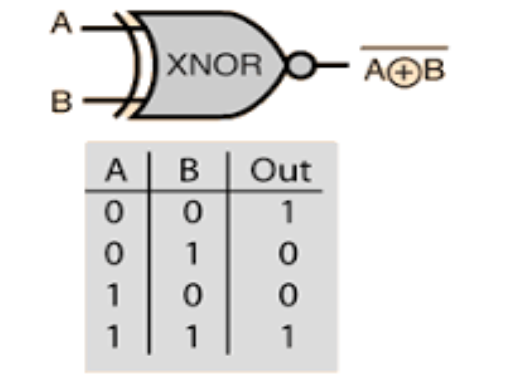
\includegraphics[scale=0.3]{tex/inc/img/xnor.jpg}
        \caption{Xnor}
    \end{center}
\end{figure}

Тогда в результате применения побитового xnor к двум бинарным векторам получается вектор, подсчет скалярного произведения из которого сводится к разности количества единиц в нем и количества нулей ($-1$ в принятом соглашении). Для подсчета количества единиц в бинарной записи числа в наборах инструкций современных архитектур ЭВМ существуют соответствующаие инструкции, такие как POPCNT в SSE4.2 Intel \cite{intel} и VCNT в Arm NEON \cite{neon}. Решив простую систему уравнений (1.9), можно получить формулу (1.10).

\begin{equation}
 \begin{cases}
 \odot = pos - neg
 \\
 size = pos + neg,
 \end{cases}
\end{equation}

\begin{equation}
 \odot = 2 pos - size
\end{equation}

где $pos$ — количество $1$ в строке, $neg$ — количество $-1$ в строке, $size$ -  размер строки в битах. 

Следовательно, результат бинарного скалярного произведения может быть посчитан с использованием (1.10) при помощи описанных выше побитовых операций. Формула (1.11) — бинарное скалярное произведение 2-ух строк матриц закодированных весов.

\begin{equation}
b^x_{i} \odot b^w_{j} = 2 popcnt(\lnot(b^x_i \oplus b^w_j)) - size
\end{equation}

Каждая из операций в (1.11) поддержана в современных архитектурах на уровне железа, что делает эту часть скалярного произведения крайне эффективной с вычислительной точки зрения.

Эффективность предложенного метода для расчета выходов нейронов ожидается не только при выполнении нейронных сетей на классических архитекутах процессоров, но и при реализации полносвязного слоя с использованием мемристорных кроссбаров. Реализация бинарного скаляного произведения на схеме с использованием мемристорных элементов приводится в \cite{memristor}. Поскольку мемристор имеет ограниченное количество уровней проводимости, матричные произведения на кросcбарах необходимо также выполнять в дискретизованном формате, что предполагает использование низкобитовой квантизации. Исследование потери точности при уменьшении количества уровней дискретизации приведено в работе \cite{discret}, где обосновывается возможность использования кроссбаров для задач глубокого обучения.

Поскольку ЭВМ способны оперировать типами данных ограниченного размера, то при условии хранения строк бинарных матриц в виде массива 32-битных целых чисел uint32, псевдокод быстрого бинарного скалярного произведения в с++20 представлен в листинге 1.1.


\begin{lstlisting}[language=C++, caption={Пример модели с LQFullyConnected}]
int32_t bin_dot(uint32_t* b_a, uint32_t* b_w, uint32_t neurons){
  uint32_t size = (neurons + 31) >> 5; // ceil divide to 32
  int32_t pos = neurons - (size << 5);
  for(uint32_t i = 0; i < size; ++i){
    pos += std::popcount(~(b_a[i] ^ b_w[i])); // popcnt(xnor)
  }
  return (pos << 1) - neurons;
}
\end{lstlisting}

Опираясь на полученную арифметику оптимального перемножения и на соображения кэш-дружелюбности при вычислениях, принято решение хранить в квантизованных слоях веса в бинаризованном формате в виде $3$-х мерного целочисленного тензора с размерами: $(o, k, ceil(n / 32))$, где $o$ — размер выходного вектора, $k$ — количество бит для кодирования каждого веса, $n$ — размер входного вектора. Деление с округлением вверх в определении размера $3$-го измерения предусматривает случаи, когда размер входного вектора $n$ не делится на $32$ целочисленно. Базис-векторы для весов следует хранить в виде вещественного тензора размера $(o, k)$ для более эффективного доступа к ним во время вычисления аппроксимированного скалярного произведения по выведенной выше формуле, а базис-вектор для кодирования входных значений может быть представлен в виде одномерного вещественного тензора, длина которого совпадает с количеством бит на кодирование одного входного значения.

\begin{figure}[H]
    \begin{center}
        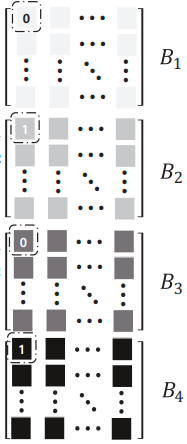
\includegraphics[scale=0.35]{tex/inc/img/bindata.jpg}
        \caption{Бинарные веса для 4 нейронов}
    \end{center}
\end{figure}

Как нетрудно догадаться, на вход слоя поступает матрица в неквантизованном виде, потому что входной вектор слоя напрямую зависит от тех вещественных данных, что приходят на вход всей нейронной сети, что делает невозможным квантизацию входов до начала исполнения модели и вынуждает проводить преобразование в бинарное представление во время работы нейронной сети каждый раз перед вычислением выходов нейронов слоя. Это является одним из существенных недостатков алгоритма, но даже несмотря на это этот казус, алгоритм остается крайне эффективным, поскольку время, которое тратится на квантизацию можно асимптотически оценить как O(n k), поскольку для каждого входного значения определяется набор бит, которые оптимально его кодирует с помощью бинарного поиска по массиву порогов квантизации, что делается за $O(log(2^K)) = O(K)$, после чего квантизованное значение записывается побитово в  буффер, на что также требуется $O(K)$ по времени.

Ранее уже было упомянуто, что задача квантизации — как можно сильнее снизить потери от перевода значений из области действительных чисел в целые числа. Для достижения этой цели базис-векторы обучаются таким образом, чтобы минимизировать ошибку между реальным вещественным значением и соответствующим его квантизованному значению действительным числом. Пусть $Q(x)$ - функция-квантизатор, которая возвращает для действительного числа $x$ его оптимальный уровень квантизации. Тогда, если описать решаемую описываемым инструментом проблему более формально, то нам необходимо найти оптимальный квантизатор, который минимизирует математическое ожидание квадратической ошибки для параметра, распределённого с плотностью $p(x)$.

\begin{equation}
Q^{*} = \argmin \limits_Q \int \limits_{- \infty}^{\infty} p(x) (Q(x) - x)^2 dx
\end{equation}

Решение этой проблемы аналитически почти всегда невозможно из-за того, что закон распределения  генеральной совокупности параметров при квантизации не известен, а поиск решения этой проблемы через линейный поиск по параметрам квантизации может занять слишком много времени. Поэтому в этом методе предлагается использовать эвристический алгоритм QEM(Quantization Error Minimization). Этот алгоритм, описание которого приводится в \cite{lq}, работает с исходным вещественным вектором входных данных $x$ и итеративно пытается улучшить значение базис-вектора $a$, основываясь на наилучшем значении этого вектора для промежуточной кодировки  $B$.

Алгоритм QEM:
\begin{enumerate}[label=\arabic*.]
    \item Инициализировать $a$ случайными значениями.
    \item Повторять от $0$ до $T$:
    \begin{enumerate}[label=\arabic*.]
    \item Найти оптимальную промежуточную кодировку $B^*$ для $x$ на основе $a$.
    \item Найти оптимальный $a^* = \argmin \limits_a \| B^* a - x \|^2$ и обновить $a$ полученным значением $a^*$.
    \end{enumerate}
\end{enumerate}

Поиск оптимальной матрицы в пункте 2.1 определяется процессом квантизации с использованием порогов, который был описан выше. Что касается пункта 2.2, то при справедливости условий Маркова-Гаусса (что на практике, к сожалению, не часто выполняется) оптимальный базис-вектор может быть найден при помощи метода наименьших квадратов по формуле (1.13), что и предлагается в \cite{lq}. 

\begin{equation}
a^* = (B B^T)^{-1} Bx
\end{equation}

Так как операция обращения матрицы является вычислительно емкой и трудно гарантировать, что определитель матрицы ковариаций $B B^T$ не будет равен или близок к $0$ в процессе обучения, поэтому в данной работе предлагается использовать итеративный градиентный спуск с $L_2$ регуляризацией, на каждой итерации которого значения будут обновляться следующим образом по формуле (1.14).

\begin{equation}
a = a - \frac{lr}{n} \sum \limits_{i = 1}^{n} [((b_i, a) - x_i)b_i + \lambda a],
\end{equation}

где $b_i$ - $i$-ый столбец матрицы $B$, $а$ - темп обучения, который задается в качестве гиперпараметра и регулирует скорость сходимости алгоритма к оптимуму. Регуляризация с параметром $\lambda$ используется чтобы штрафовать большие значения параметров, потому что веса и входы слоёв, как правило, имеют небольшие значения.

Применение данного алгоритма для обучения базис-вектора параметров предлагается в данной работе как основа инструмента для post-training квантизации. Этот метод обучения работает не только в предлагаемом методе работы с весами и активациями слоя. Он может определять оптимальные значения параметров для других методов, например BiQGEMM из \cite{bqgemm},  в котором предлагается иной способ  расчета результата генерального матричного произведения без перевода входных значений в целочисленный вид, но совпадает формат хранения и интерпретация весов слоя. 